\documentclass[
10pt, % Main document font size
letterpaper, % Paper type, use 'letterpaper' for US Letter paper
oneside, % One page layout (no page indentation)
%twoside, % Two page layout (page indentation for binding and different headers)
headinclude,footinclude, % Extra spacing for the header and footer
BCOR5mm, % Binding correction
]{scrartcl}

\usepackage[spanish]{babel}

%%%%%%%%%%%%%%%%%%%%%%%%%%%%%%%%%%%%%%%%%
% Arsclassica Article
% Structure Specification File
%
% This file has been downloaded from:
% http://www.LaTeXTemplates.com
%
% Original author:
% Lorenzo Pantieri (http://www.lorenzopantieri.net) with extensive modifications by:
% Vel (vel@latextemplates.com)
%
% License:
% CC BY-NC-SA 3.0 (http://creativecommons.org/licenses/by-nc-sa/3.0/)
%
%%%%%%%%%%%%%%%%%%%%%%%%%%%%%%%%%%%%%%%%%

%----------------------------------------------------------------------------------------
%	REQUIRED PACKAGES
%----------------------------------------------------------------------------------------

\usepackage[
nochapters, % Turn off chapters since this is an article        
beramono, % Use the Bera Mono font for monospaced text (\texttt)
eulermath,% Use the Euler font for mathematics
pdfspacing, % Makes use of pdftex’ letter spacing capabilities via the microtype package
dottedtoc % Dotted lines leading to the page numbers in the table of contents
]{classicthesis} % The layout is based on the Classic Thesis style

\usepackage{arsclassica} % Modifies the Classic Thesis package

\usepackage[T1]{fontenc} % Use 8-bit encoding that has 256 glyphs

\usepackage[utf8]{inputenc} % Required for including letters with accents

\usepackage{graphicx} % Required for including images
\graphicspath{{Figures/}} % Set the default folder for images

\usepackage{enumitem} % Required for manipulating the whitespace between and within lists

\usepackage{lipsum} % Used for inserting dummy 'Lorem ipsum' text into the template

\usepackage{subfig} % Required for creating figures with multiple parts (subfigures)

\usepackage{amsmath,amssymb,amsthm} % For including math equations, theorems, symbols, etc

\usepackage{varioref} % More descriptive referencing

%----------------------------------------------------------------------------------------
%	THEOREM STYLES
%---------------------------------------------------------------------------------------

\theoremstyle{definition} % Define theorem styles here based on the definition style (used for definitions and examples)
\newtheorem{definition}{Definition}

\theoremstyle{plain} % Define theorem styles here based on the plain style (used for theorems, lemmas, propositions)
\newtheorem{theorem}{Theorem}

\theoremstyle{remark} % Define theorem styles here based on the remark style (used for remarks and notes)

%----------------------------------------------------------------------------------------
%	HYPERLINKS
%---------------------------------------------------------------------------------------

\hypersetup{
%draft, % Uncomment to remove all links (useful for printing in black and white)
colorlinks=true, breaklinks=true, bookmarks=true,bookmarksnumbered,
urlcolor=webbrown, linkcolor=RoyalBlue, citecolor=webgreen, % Link colors
pdftitle={}, % PDF title
pdfauthor={\textcopyright}, % PDF Author
pdfsubject={}, % PDF Subject
pdfkeywords={}, % PDF Keywords
pdfcreator={pdfLaTeX}, % PDF Creator
pdfproducer={LaTeX with hyperref and ClassicThesis} % PDF producer
} 
\hyphenation{Fortran hy-phen-ation}

\title{\normalfont\spacedallcaps{Banco de Datos INMEGEN}}
\author{\spacedlowsmallcaps{Rodrigo García Herrera}}
\date{} % An optional date to appear under the author(s)



\begin{document}

%----------------------------------------------------------------------------------------
%	HEADERS
%----------------------------------------------------------------------------------------

\renewcommand{\sectionmark}[1]{\markright{\spacedlowsmallcaps{#1}}} % The header for all pages (oneside) or for even pages (twoside)
%\renewcommand{\subsectionmark}[1]{\markright{\thesubsection~#1}} % Uncomment when using the twoside option - this modifies the header on odd pages
\lehead{\mbox{\llap{\small\thepage\kern1em\color{halfgray} \vline}\color{halfgray}\hspace{0.5em}\rightmark\hfil}} % The header style

\pagestyle{scrheadings} % Enable the headers specified in this block


%----------------------------------------------------------------------------------------
%	TABLE OF CONTENTS & LISTS OF FIGURES AND TABLES
%----------------------------------------------------------------------------------------

\maketitle % Print the title/author/date block
\setcounter{tocdepth}{2} % Set the depth of the table of contents to show sections and subsections only
\tableofcontents % Print the table of contents
%\listoffigures % Print the list of figures
%\listoftables % Print the list of tables



%%%%%%%%%%%%
% The text %
%%%%%%%%%%%%

\section{Antecedentes}


\subsection{Open Science, Open Data}

Los datos constituyen la evidencia del conocimiento científico. Más
datos disponibles significan mayor nivel de transparencia y
reproducibilidad. Asegurarse de que los datos estén ampliamente
disponibles a la comunidad científica acelera el ritmo de la
investigación y mejora su eficiencia. \cite{walport_sharing_2011}

Compartir datos detallados -incluyendo atributos de muestras, factores
y resultados clínicos, secuencias genómicas, datos crudos de
microarreglos- con otros investigadores permite que estos recursos
contribuyan más allá de los análisis originales.

Además de usarse para confirmar resultados originales, los datos
crudos pueden usarse para explorar hipótesis nuevas o relacionadas,
tanto más cuando se combinan con otros conjuntos de datos públicos.
Uno de los aspectos más interesantes de compartir datos es que
cualquiera en desacuerdo con las elecciones analíticas de los primeros
autores puede usar modelos alternativos, u otra selección de datos y
posiblemente llegar a diferentes conclusiones.

Tener datos reales es indispensable al investigar y desarrollar
métodos de estudio, técnicas de análisis e implementaciones de
software. La comunidad científica en general también se beneficia:
compartir datos promueve múltiples perspectivas, ayuda a identificar
errores, disuade de conductas fraudulentas, es útil para el
entrenamiento de nuevos investigadores y aumenta la eficiencia en el
uso de fondos y poblaciones de pacientes al evitar la colección
duplicada de datos.\cite{piwowar_sharing_2007}

Algunas barreras que dificultan la publicación de datos son: falta de
infraestructura informática, restricciones impuestas por los autores,
publicación de datos difíciles de reusar por estar pobremente anotados
o imposibles de extraer (por ejemplo datos en tablas de archivos
PDF).\cite{molloy_open_2011}.

Este documento es una propuesta para la creación de un Banco de Datos
Genómicos tal que elimine los obstáculos para la diseminación y
archivado de los datos que acompañan a las publicaciones del INMEGEN.


\subsection{Datos en el INMEGEN}



\section{Objetivos y alcance}


\subsection{Banco de datos}

Diseño e implementacion de un sistema informático que permita a
investigadores del INMEGEN compartir datos de manera uniforme etc. con
la comunidad científica. Que permita a la comunidad científica obtener
datos publicados por el instituto. Que ayude a establecer vínculos y a
medir el impacto de los datos. Que cumpla con estándares: formatos,
respaldos, replicación, catálogos.
\cite{_data_????}
\cite{altman_proposed_2007}



\subsection{Interfaces Global Alliance for Genomics and Health}

El grupo de trabajo de Datos de la Global Alliance for Genomics and
Health a producido múltiples piezas de software para el
aprovisionamiento de interfaces de intercambio de datos. El Banco de
Datos del INMEGEN podría implementarlas para maximizar su
interoperabilidad.

\subsubsection{Matchmaker Exchange}

El esfuerzo colaborativo \em{Matchmaker Exchange}\em  enfrenta el reto de la
falta de claridad en la etiología en la mayoría de las muestras a las
que se les secuencia el exoma o el genoma, tanto en ámbitos clínicos
como académicos. En estos casos el hallazgo de un sólo caso adicional
con una variante deleterea en el mismo gen y el mismo fenotipo puede
ser evidencia suficiente para identificar el gen causal. Múltiples
laboratorios y consorcios que investigan enfermedades raras colectan
datos de manera independiente, lo que resulta en esfuerzos
fragmentados que dificultan la agregación de casos similares.

Este proyecto pretende crear una red confederada de infraestructura
que permita hallar pacientes similares a través de diferentes bases de
datos, en especial para facilitar el descubrimiento de las causas
genéticas de enfermedades raras. La red de bases de datos se
interconecta a través de la Matchmaker Exchange API, una interfaz
programática para hacer búsquedas de pacientes a través de sus
perfiles fenotípicos y genotípicos.\cite{_matchmaker_????}


\subsubsection{Beacon Project}
Se trata de un servicio público a través de la web que cualquier
institución puede implementar. Simplemente acepta preguntas como:
¿tienen genomas con la base 'A' en la posición 100,735 en el cromosoma
3? (y del estilo) y responde con ``sí'' o ``no''.

Es simple desde el punto de vista técnico, y no devuelve más
información. El objetivo de implementar un ``Beacon'' es mostrar
disponibilidad al diálogo e intercambio de datos con otras
instituciones.\cite{_ga4gh_????}


\subsubsection{Genomics API}

Esta interfaz programática permitirá el intercambio e
interoperabilidad sobre información genómica a través de múltiples
organizaciónes y múltiples plataformas. Es un estandar libre y abierto
que usa protocolos web para dar soporte a la transmisión de datos de
secuencias de ADN y de variación genómica. La interfaz permite la
creación de fuentes de información que puede integrarse a software de
visualización, a portales web de datos genómicos o a \em{pipelines}\em
de análisis. Se sobrepone a barreras de infraestructura incompatible
entre organizaciones e instituciones para facilitar el intercambio de
datos de ADN a quienes los proveen y quienes los consumen.\cite{_ga4gh_????-1}

La figura \vref{fig:interop} muestra diferentes programas accediendo a
diferentes repositorios de datos a través de la Genomics API.

\begin{figure}
\centering 
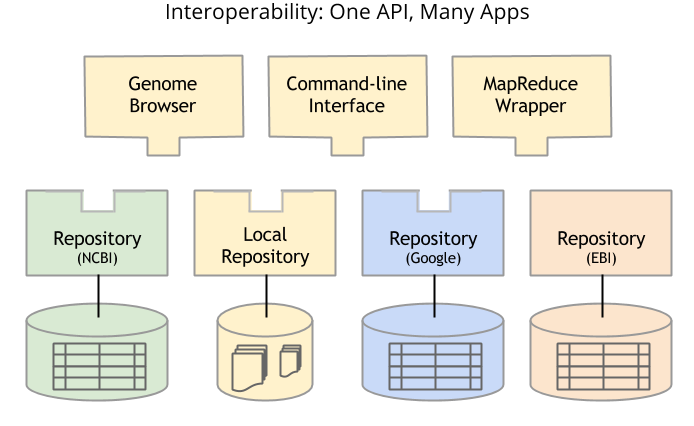
\includegraphics[width=0.8\columnwidth]{GA4GH_API_interop.png} 
\caption[]{Interoperación de repositorios de datos y programas a
  través de la Genomics API}
\label{fig:interop} 
\end{figure}



\subsection{Enlaces con otros Repositorios}
Establecer un proceso que permita identificar repositorios públicos
con mayor masa crítica para ciertos tipos de datos.

Establecer un proceso que permita identificar cuáles de nuestros datos
van en esos repositorios.
\cite{_genebank_????}
\cite{king_introduction_2007}

Gene expression omnibus

\section{Justificación}

\subsection{Publicación de datos.}


\subsubsection{Requisito de Revistas}

Algunas revistas, incluyendo la familia PLoS, requieren la sumisión de
datos biomédicos detallados a bases de datos públicas como condición
para publicar en ellas.\cite{piwowar_sharing_2007, hrynaszkiewicz}

Otras agencias como el National Institute of Heath (NIH), la National
Science Foundation (NSF), el Wellcome Trust, el Medical Research
Council (MRC), la Deutsche Forschungsgemeinschaft (DFG) estipulan que
grantees deben tener un plan para compartir datos como parte de sus
propuestas o publicar sus datos al completar sus
proyectos.\cite{wicherts_publish_2012}

Tener un banco de datos institucional y mecanismos institucionales
para la publicación de datos en repositorios establecidos facilitará
el cumplimiento del requisito de publicación de datos que
habitualmente es política de estas revistas donde publicamos.


\subsubsection{Citación}
Es una decisión razonable de los editores requerir a sus autores
que provean acceso a los datos: aquellos artículos en revistas con
políticas de replicación que dan acceso a los datos se citan con tres
veces más frecuencia que sus equivalentes sin datos.\cite{walport_sharing_2011}


\subsubsection{Reproducibilidad, transparencia}
La ciencia reproducible es de mayor calidad y redunda en más exposición y
citación. \cite{piwowar_sharing_2007, ioannidis_improving_2011}

Institutos e investigadores deben asegurarse de soportar no sólo el
hardware necesario para almancenar los datos, sino también el software
que permite analizarlos. Un aspecto importante es el software para
manejo de metadatos: herramientas que facilitan el proceso de
anotaciónn de los datos con descripciones de lo que significan sus
diferentes partes, con qué instrumento se colectaron, qué algoritmos
se les han aplicado, etc. Esta información es esencial para que otros
científicos en efecto puedan reusar los datos. Toda esta información
debe hospedarse y ser asequible a largo plazo. Quizá las mismas
bibliotecas pueden tomar este rol.\cite{said_datas_2009}


\subsubsection{Política de Datos Abiertos}
El Programa para un Gobierno Cercano y Moderno (PGCM) 2013-2018
instaura una Política de Datos Abiertos.

La Unidad de Gobierno Digital provee infraestructura para un catálogo
central, pero el hospedaje de los datos debe proveerse por las
instituciones que las publican.

Para cumplir con estos requisitos en la actualidad el INMEGEN publica
datos a través del portal \url{http://genomamexicanos.inmegen.gob.mx} que
brinda acceso al explorador del HapMap con la aplicación
\url{http://diversity.inmegen.gob.mx/} y a los datos crudos de microarreglos
en \url{http://data.inmegen.gob.mx/}.

Sin embargo se trata de un sólo estudio y sería insuficiente como
catálogo de datos para otras plataformas genómicas. Un banco de datos
permitiría cubrir los requisitos de la Política de Datos Abiertos para
datos de más estudios.


\subsection{Vinculación, colaboración}
Compartir datos da ocasión de establecer contacto con organizaciones e
individuos interesados en las mismas líneas de investigación.

Algunos tipos de investigación ganan gran poder estadístico con la
inclusión de más pacientes, mendelian, (citar acá global alliance
mendelian). 


\section{Metodología}


\subsection{Creación de Grupo de trabajo}


\subsection{Inventario Institucional}
\cite{_nih_????}

\subsection{Publicación}
Repositorios externos.
APIs.
Página web, catálogo en línea, bit-torrent.

\subsection{Promoción}
\cite{schofield_post-publication_2009}


%----------------------------------------------------------------------------------------
%	BIBLIOGRAPHY
%----------------------------------------------------------------------------------------

\renewcommand{\refname}{\spacedlowsmallcaps{References}} % For modifying the bibliography heading

\bibliographystyle{unsrt}

%\bibliography{sample.bib}
\bibliography{inmegen_databank}

%----------------------------------------------------------------------------------------

\end{document}